% Chapter 2

\chapter{Data} % Write in your own chapter title
\label{Chapter2}
\lhead{Chapter 2. \emph{Data}} % Write in your own chapter title to set the page header

In this chapter I discuss the data, surveys and the follow-up facilities used in this thesis. I begin by discussing the Supernova Legacy Survey (SNLS) which was used in the early part of this thesis and was the source of data for my work on the rate of SLSNe at z$\sim$1, discussed further in \cref{Chapter3}. Following from this I discuss the Dark Energy Survey (DES) which provided a bigger and higher redshift sample of transients used in my search for high redshift SLSNe as described in \cref{Chapter5}. I then give a brief overview of the follow-up facilities used in the classifying of SLSNe that were discovered in real time using the techniques discussed in \cref{Chapter5}. Finally I describe the process of collecting and unifying the sample of published SLSNe used as a baseline dataset throughout this work.

\section{Supernova Legacy Survey}
The Supernova Legacy Survey \citep{Boulade2003MegaCam:Camera,Pritchet2004SNLSSurvey} was run as part of the Canadian-French-Hawaii Telescope Legacy Survey (CFHT-LS) between 2003 and 2008. Over that time it has proven to be one of the most successful SN surveys to date, observing thousands of transients and spectroscopically confirming a large proportion of that including over 300 SN-Ia \citep{Perrett2010Real-timeSurvey}, XX core-collapse supernovae as well as measuring giving one of the best measurements of their respective rates \citep{Perrett2012EVOLUTIONSURVEY} [CITE CC RATE]. SNLS has also discovered two SLSNe at z=1.588 and z=1.50 \citep{Howell2013TwoSurvey} which, until recently, have been the highest redshift, spectroscopically identified objects of this class to date. The principle objective of the survey was to perform a measurement of the cosmological constants $\omega_{\Lambda}$ and $\omega_{m}$ \citep{Sullivan2011SNLS3:PROBES,Astier2013PhotometrySNLS}. This resulted in a great success producing the most precise measurement until the Planck era in a joint analysis with the WMAP survey. This was in a large way made possible thanks to the observing strategy optimized to maximize the number of high redshift SN-Ia candidates and the thorough spectroscopic follow-up program which gave a much stronger constrains for the Hubble diagram fits thanks to the high-z leverage not possible before with low redshift SN-Ia surveys.

\subsection{Survey Overview}
SNLS used the 4m Canadian-French-Hawaiian Telescope (CFHT) situated on Mauna Kea, Hawaii. It was operated by two teams from Canada and France as part of the CFHT Legacy Survey that composed of a small area, deep SN survey and a shallow, wide galaxy survey aimed at studying the large scale structure of the Universe and the cosmological parameters though the galaxy clustering and weak lensing. Four, $\sim$1 deg$^2$ deep fields have been observed to the limiting magnitude of m=23.5 using the 400 megapixel MegaCam camera \citep{Boulade2003MegaCam:Camera}. Observations took place over five seasons, each lasting approximately 5 months. In total 202 nights have been allocated to the survey \citep{Pritchet2004SNLSSurvey}.

\subsection{Cadence and Observations}
SNLS carried out the observations in the \textit{griz} photometric bands, similar in bandpass to the filters used in SDSS \fref{fig:SNLSFilters}. Each field was observed with an average cadence of 5 days [CITE AND CHECK] covering all bands on the same night if the conditions have observing conditions allowed for this. As a survey aimed at producing the most densely populated, high quality Hubble diagram, the cadence was optimized to maximize the number of detections of SN-Ia at mid to high redshift (0.3 $\leq$ z $\leq$ 1.0) with a sufficient data quality to light curve model fitting [CITE]. In the late stages of each season this strategy was sometimes altered slightly to focus on follow-up of already detected SN-Ia in the redder bands rather than detecting new candidates in the blue bands.

\begin{figure}
  \centering
  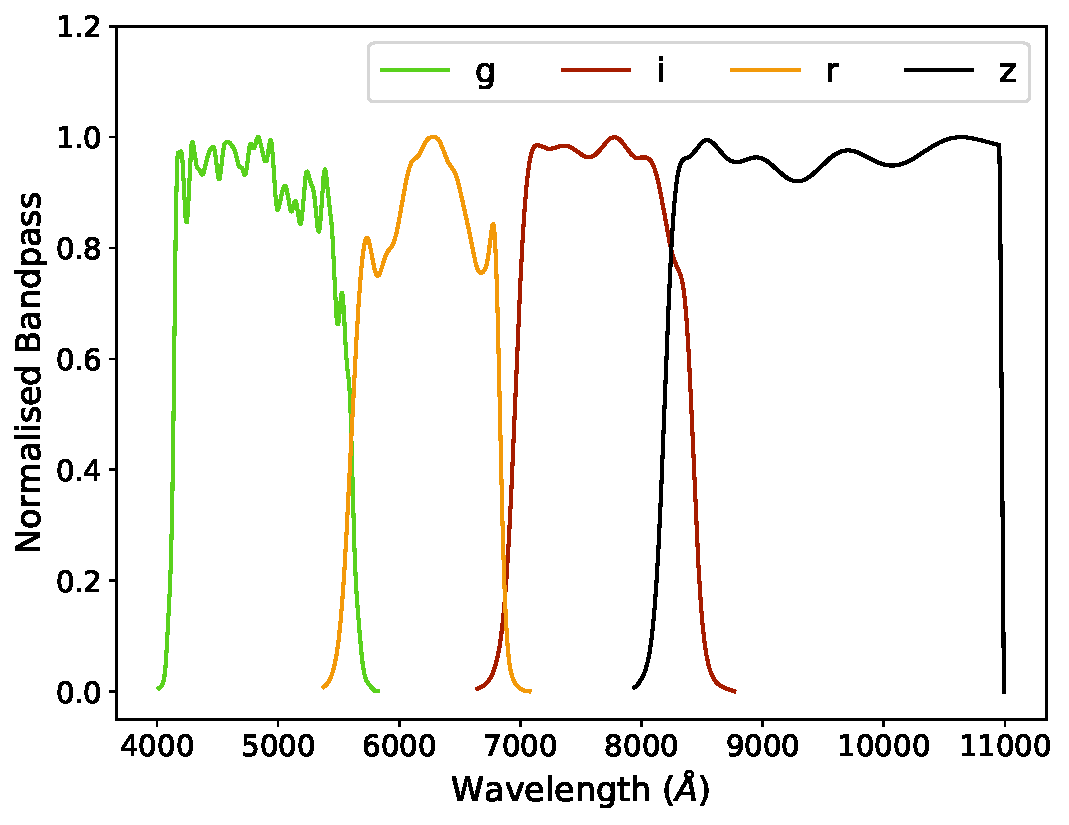
\includegraphics[scale=0.8]{Figures/Chapter2/SNLS_filters.pdf}
	\caption{Bandpass response for filters used in SNLS compared to a 				spectrum of a SLSN; SNLS06D4eu at z=1.588 discovered by the 			  survey [TODO]}
    \label{fig:SNLSFilters}
\end{figure}

\subsection{Data Reduction}
Several different data reduction pipelines have been used in the analysis of the SNLS data. In this thesis we used a combination of data prepared for public and internal data releases, as well as reanalysis of data using PTFPhot, a custom, pre-existing pipeline designed to improve the data reduction quality \citep{Firth2015TheSupernovae}.

\paragraph{Real-time photometry}
During the live operations of the survey the pre-processed data has been independently analyses by the French and Canadian teams using separate quick-reduction pipelines \citep{Bazin2011} [CITE MORE]. Both teams aimed to produce lists of newly, viable SN candidates within hours of their observations before forwarding them to the spectroscopic follow-up facilities. Both teams were very successful and produced mostly identical lists which lead to high classification accuracy, subsequently leading to the success of the survey \citep{Pritchet2004SNLSSurvey}.\\

\paragraph{Forced photometry}
The quick reduction pipeline used in the detection of objects was optimized with speed, rather than accuracy, in mind. Any scientific analysis of the data requires a much higher accuracy of the photometry. The data for 'real' transient, defined as as having detections on multiple epochs and in multiple bands, is passed though a much improved, custom ,forced photometry pipeline; PTFPhot \citep{Firth2015TheSupernovae}. The primary improvements in this code over the quick photometry come from full and proper modeling of the PSF of each image as well precisely measuring the position of the SN in the full stack of images and subsequently extracting the PSF photometry at that position in each individual image (giving the 'Forced' name). This largely decreases the uncertainties associated with the flux measurement, especially for faint sources close to or below the detection limit. This analysis has been applied to the data in the data releases that provided the source of data for the work in \cref{Chapter3} and other analysis such as the rates of SN-Ia \citep{Perrett2012EVOLUTIONSURVEY}, core-collapse SN \citep{Bazin2009} as well as the early cosmological results \citep{Sullivan2011SNLS3:PROBES}. \\
 
\subsection{Spectroscopic Follow-Up}
The success of SNLS cannot be attributed only to the the number of transients discovered by the survey but also to the effort behind the spectroscopic follow-up of the candidates. Between the Very Large Telescope (VLT), Keck, Gemini North and South and Magellan XXX hours have been allocated for spectroscopic follow-up. This in total has, in fact, exceeds the time allocated to SNLS itself. As a result XXX SN-Ia have been spectroscopically confirmed [CITE] along with xx CCSN [CITE] and two SLSNe \citep{Howell2013TwoSurveyb}

\subsection{Redshift measurements}
A key part of any SN analysis is their distance measurement. SNLS provided three types of redshift sources: SN spectroscopic redshift, host galaxy spectroscopic redshift and photometric redshift estimates from host galaxy template fitting. In both spectroscopic cases, the redshift is measured using galaxy emission line features and are often extremely precise as they require multiple line identifications as long as the signal-to-noise ratio and resolution of the data allows for this. We can therefore assume the values to be correct and reliable.

\subsection{SLSN in SNLS}
SNLS was not an ideal survey for detecting SLSN. Do to the primary objective of the project being the study of SN-Ia, its focus on a small area and relatively dense cadence meant that the volume searched was not sufficient to the detect a large number of SLSN, known to be a very rare class of astronomical events \citep{Cooke2012Superluminous3.90.,Prajs2017The1,Quimby2013Rates0.2}. Despite this, two events have been discovered; SNLS07D2bs at z=1.50 and SNLS06D4eu at z=1.588 with the remaining as the highest redshift SLSN discovered for a full decade until this record was taken by DES.

Furthermore, after the completion of the survey from individual seasons have been co-added together to create "super" stacks reaching a detection magnitude of m=26.5 \citep{Cooke2012Superluminous3.90.}. Two objects have been detected using this technique that had a light curve behavior similar to that of a SLSN. While it was impossible at that point (several years after the live transient) to spectroscopically identify these objects, host galaxy spectroscopy was obtained for both objects determining redshifts of z=2.05 and z=3.9 \citep{Cooke2012Superluminous3.90.}. This also confirmed that the transients had a luminosities comparable to that of SLSN. While these candidate SLSNe show an interesting precedent for what may be hiding beyond the reach of our current, 4m telescope class, optical surveys, they were not used in any projects within this thesis. The lack of certain confirmation, low cadence in the stacked images light curve and the difference in the detection technique used deemed these objects incompatible with other SLSN data sources \citep{Prajs2017The1}.

\section{Dark Energy Survey}
The Dark Energy Survey (DES) is the largest cosmology survey operated to date. It is composed of two elements; a wide galaxy survey and a SN component. It's main aim is to perform the most precise, to date, measurement of the cosmological parameters.

\subsection{Survey Setup}
DES uses a purpose build XXX mega-pixel DECam camera mounted on the 4m Blanco telescope at the Cerro-Tollolo observatory in Chile. One of the greatest advantages of DECam over its predecessors is its high sensitivity at red wavelengths allowing for high signal to noise observations in \textit{z} and \textit{y} bands. DES was awarded 500 observing nights over the period of 5 years between 2013 and 2018. Each observing seasons starts in late August and ends at the end of January giving on average a 5 months long observing period.

\paragraph{Wide Survey}
DES wide survey has been designed to observe 5000 deg$^2$ of the southern sky to the depth of m$\sim$25 in the \textit{ugrizy} filters. The aim of this is to create the largest catalog of galaxies and their associated redshifts to date at an unprecedented resolution and depth with the first public data release contained a catalog of 400 million galaxies from the initial 3 years of the survey. These data can be used to study cosmology via three separate experiments; the Baryon Acoustic Oscillations (BYO), Galaxy Clustering and Weak Lensing [CITE ALL].

\paragraph{Supernova Survey}
The SN survey as part of DES is a dedicated search optimized to study and discovered the highest number of SN-Ia to date. To maximize the number of discovered SN-Ia 10 fields are observed in the \textit{griz} photometric bands. Eight of these fields are 'shallow' and observe to the depth of m=23.5 while two fields have been chosen to be 'deep' and observe to m=25. The number of deep and shallow fields was chosen as an optimal value that allowed for the largest number of SN-Ia to be discovered at the same time searching for high redshift objects at z>1 [CITE].

The cadence of the DES

As the the Weak Lensing experiment of the wide survey requires very good seeing images in order to resolve the shapes of galaxies, it is that component that receives a priority over the best quality night. In case where the observations are

\subsection{Photometric Redshifts}
With the vast quantities of galaxies detected by DES it is not currently possible, even with the largest integrated field spectrograph, to obtain spectroscopic redshifts for even a small fraction of these objects. A photometric approach must be used to achieve the overall cosmological goals of the survey. While most DES observations are carried out using the \textit{griz} filters \textit{u} and \textit{y} are used, albeit at a lower depth, to aid with the galaxy SED template fitting used to estimate the redshifts. This method is not particularly accurate at low redshifts, however it becomes sufficiently precise at z>0.3 [CITE]. This is due to the steep oxygen[??] drop at 4000\AA [??] shifting into the redder bands amongst other galaxy features.


\section{SUDSS}
The Search Using DECam for Superluminous Supernovae (SUDSS) (PI: Sullivan) was designed as a dedicated SLSN survey working in conjunction with DES. Its aim was to extend the DES observing season from 6 months to $\sim$ 9 months by observing the fields at high airmass until the observations become impossible due the sun constrains. While, do to technical issued \sref{sec:SUDSSIssues}, it has never been used as a tool for searching for new SLSN candidates it has greatly enhanced the light curves of some SLSNe discovered by DES.

\subsection{Observations and Data Reduction}
SUDSS observed XX fields between the end of 1st DES season and start of the 4th season (Periods Pxx to Pxx). The observations were carried out using DECam with an identical setup to DES allowing for the same pre-processing steps to be applied to the data. The data was not directly fed into the DES database nor did it use the force photometry pipeline used by DES for technical reasons. Instead the data was reduced using a custome PTFPhot pipeline [CITE ROB]. For the purpose of unbiased comparison, corresponding DES observations of the SUDSS SLSNe were also reduced using the PTFPhot pipeline.

\subsection{Cadance and Exposures}
\label{sec:SUDSSCadance}
SUDSS was designed with the aim of discovering new SLSN candidates at its very heart. It was initially believed [CITE] that it will be capable of identifying $\sim$ 100 SLSN candidates during its operation. As SLSN are a class of slowly evolving supernova, the DES observing cadance was not retained for SUDSS and instead it was chosen to be two weeks. Due to worse that anticipated weather conditions many of these nights have been lost to cloudy nights resuting in a final cadance closer to 1 month. On avarage three additional observations were made in each field outside of the DES observing season.

A futher difference between the DES and SUDSS observing strategies comes in the exposure times used for the observations. As SLSN are much brighter but rarer events than SN-Ia (which are the main focus of the DES SN survey) the exposure times did not have to match that of the DES deep fields to still search for SLSNe at redshifts greater than z>1, however, they did exceed the relatively short exposure times of DES shallow SN field. In practice the limitig magnitude of SUDSS was similar to that of the DES shallow fields once the unfavorable atmospheric conditions and high air mass have been taken into account.

\subsection{Findings}
\label{sec:SUDSSIssues}
As a result of the poor cadance and lower than expected image quality it was not possible to carry out a dedicated search for SLSN in the SUDSS data alone. Instead, the SUDSS data have been repurposed as an auxilary data source for objects already discovered by DES. This has been extremely sucessful and resulted in a great improvemnt to the light curves of some of the SLSNe discoved by DES. In cases of DES15C3hav and DES15X2hm we were able to determine the explosion date and hence contrain the rise time of these SNe using the SUDSS data points.

The most significant observations came in form of DES14X3taz [CITE MAT] where the auxilary SUDSS data provided the observations of the pivotal rise and peak of this unique "bumpy" SLSN. Without the SUDSS observations a large proportion of the analysis carried out in [CITE] would have not been possible.

\section{DES Spectroscopic Follow-up Facilities}

\section{Literature sample of SLSNe}
Throughout this thesis a sample of SLSN, published in years between 2010 and 2016, has been used to define what a SLSN is. We define SLSN as any hydrogen poor SLSN and do not distinguish between slowly and rapidly evolving objects [CITE INSERRA AND GAL-YAM]. All objects come from a variety of surveys which includes xx PTF, 1 iPTF, 2 SNLS, 3 DES and xx PS1 SNe. The broad mix of surveys means that the objects are not of the same quality, are not in the same photometric systems and do not use the same band passes.

\subsection{Quality cuts}
We devised a set of quality cuts to ensure that the objects used in our analysis meet a minimum standard. As most of our analysis, discussed in the forthcoming chapters, depends on fitting black bodies to the light curve we require that the light curve must contain a minimum of three distinct photometric bands, i.e Even thought they would be modeled independently we would count SDSS and PS1 \textit{r}-band filters as one for the purpose of the quality cut. Furthermore we make a cut on the number of epochs observed per band. In order to use models which depend on the rise and decline time of the supernova we require that there are a minimum of two photometric points before the peak and two points after the peak. As the SN evolve rapidly in temperature and hence colour, the bluer bands peak several days before redder bands. We define the peak as the maximum in the band closest to rest frame U-band. \tref{tab:PubishedSLSNe} shows the list of SLSN used throughout this work that have passed our data quality cuts.

\subsection{Converting and converging photometric systems}
It is standard practice in the SN literature to publish the photometry for studied objects in form of a table of magnitudes per band on given observing nights. Magnitude scale is not, however, the most useful when fitting models to the data. As it is logarithmic in nature, the photometric uncertainties, originally measured in the linear count space and often Gaussian in nature become asymmetric and therefore more difficult to deal with in model fitting. It is a lot easier to convert the magnitudes, M, to flux, $\nu$ using a zero point, $zp$ for a given filter:
\begin{equation}
\label{eq:MagToFlux}
\nu = 10^{-0.4 \times M~+~zp}
\end{equation}
similarly we convert the uncertainties in magnitude to flux using \eqref{eq:MagErrorToFlux}.
\begin{equation}
\label{eq:MagErrorToFlux}
\Delta \nu = 0.921034~\times~10^{-0.4 \times M~+~zp}~\times~\Delta M
\end{equation}
It is customary in literature to quote the magnitudes for the SDSS filters (\textit{ugrizy}) in the AB photometric system and the Johnson filters (\textit{UBVRIJHK}) in the Vega system. If not otherwise stated in the papers these are the systems used for the zero points in conversion between magnitude and flux. If not stated otherwise it is also assumed that the photometry has been corrected for Milky Way extinction which is a standard procedure in most modern surveys [CITE PTF, DES, SNLS etc].

\begin{table}
\begin{center}
  \caption{The training sample of SLSNe-I.}
\label{tab:PubishedSLSNe}
\begin{tabular}{|l|r|l|l|}
\hline
  \multicolumn{1}{|c|}{SN Name} &
  \multicolumn{1}{c|}{Redshift} &
  \multicolumn{1}{c|}{Survey} &
  \multicolumn{1}{c|}{Reference} \\
\hline
  PTF12dam & 0.108 & Palomar Transient Factory & \citep{2013Natur.502..346N}\\
  SN2011ke & 0.143 & Catalina Real-Time Transient Survey & \citet{2013ApJ...770..128I}\\
  &&\& Palomar Transient Factor & \\
  SN2010gx & 0.230 & Palomar Transient Factory & \cite{2010ApJ...724L..16P}\\
  SN2013dg & 0.265 & Catalina Real-Time Transient Survey & \cite{2014MNRAS.444.2096N} \\
  PS1-11ap & 0.524 & Pan-STARRS & \cite{2014MNRAS.437..656M}\\
  DES14X3taz & 0.608 & Dark Energy Survey & \cite{2016ApJ...818L...8S} \\
  PS1-10bzj & 0.650 & Pan-STARRS & \cite{2013ApJ...771...97L}\\
  DES13S2cmm & 0.663 & Dark Energy Survey & \cite{2015MNRAS.449.1215P} \\
  iPTF13ajg & 0.741 & intermediate Palomar Transient Factory &\cite{2014ApJ...797...24V}\\
  SNLS-07D2bv & 1.500 & SNLS &\cite{2013ApJ...779...98H}\\
  SNLS-06D4eu & 1.588 & SNLS &\cite{2013ApJ...779...98H}\\
\hline\end{tabular}
\end{center}
\end{table}
